%\chapter{Annexes}
\label{chap:annexes}
%\minitoc

\chapter{Caractéristique d'Euler}

La caractéristique d'Euler, formulée par le mathématicien suisse Leonhard Euler au XVIIIe siècle, joue un rôle central dans les domaines de la topologie et de la géométrie. Elle constitue un outil puissant permettant de décrire de manière élégante et efficace des objets géométriques complexes en utilisant des concepts mathématiques simples. Il s'agit d'un invariant topologique c'est à dire un nombre associé à une variété, qui est invariant par homéomorphisme (c’est-à-dire que la valeur de cet invariant est la même pour deux variétés homéomorphes).
\begin{figure}[!h]
\begin{subfigure}{0.5\textwidth}
    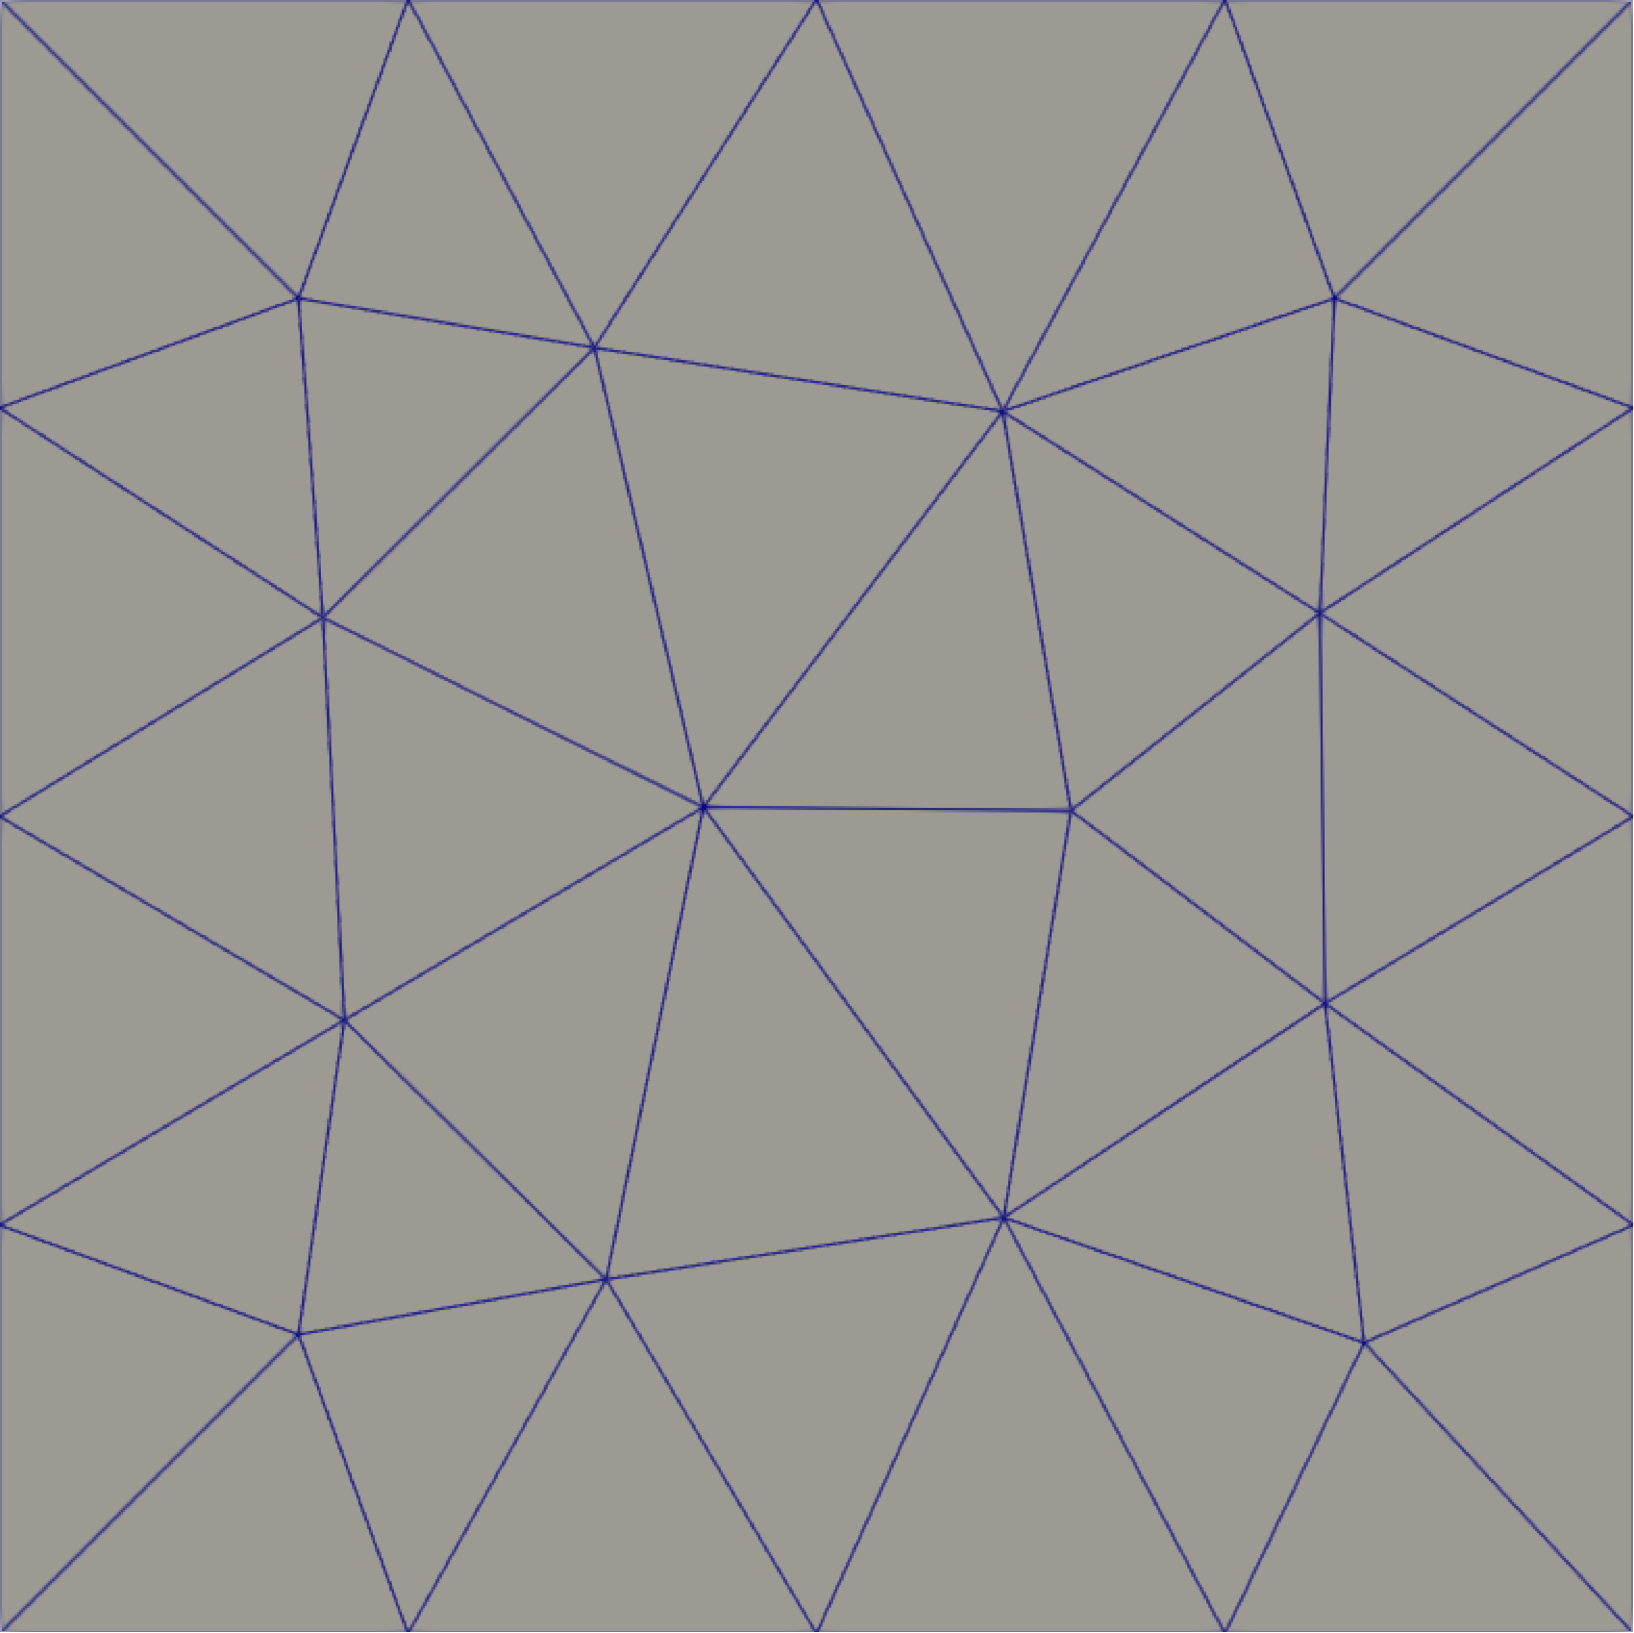
\includegraphics[width=\textwidth]{images/carre_euler_1.pdf}
    %\caption{Maillage triangulaire.}
    %\label{fig:mail_tri_vs_mail_quad_1}
\end{subfigure}
\hfill
\begin{subfigure}{0.5\textwidth}
    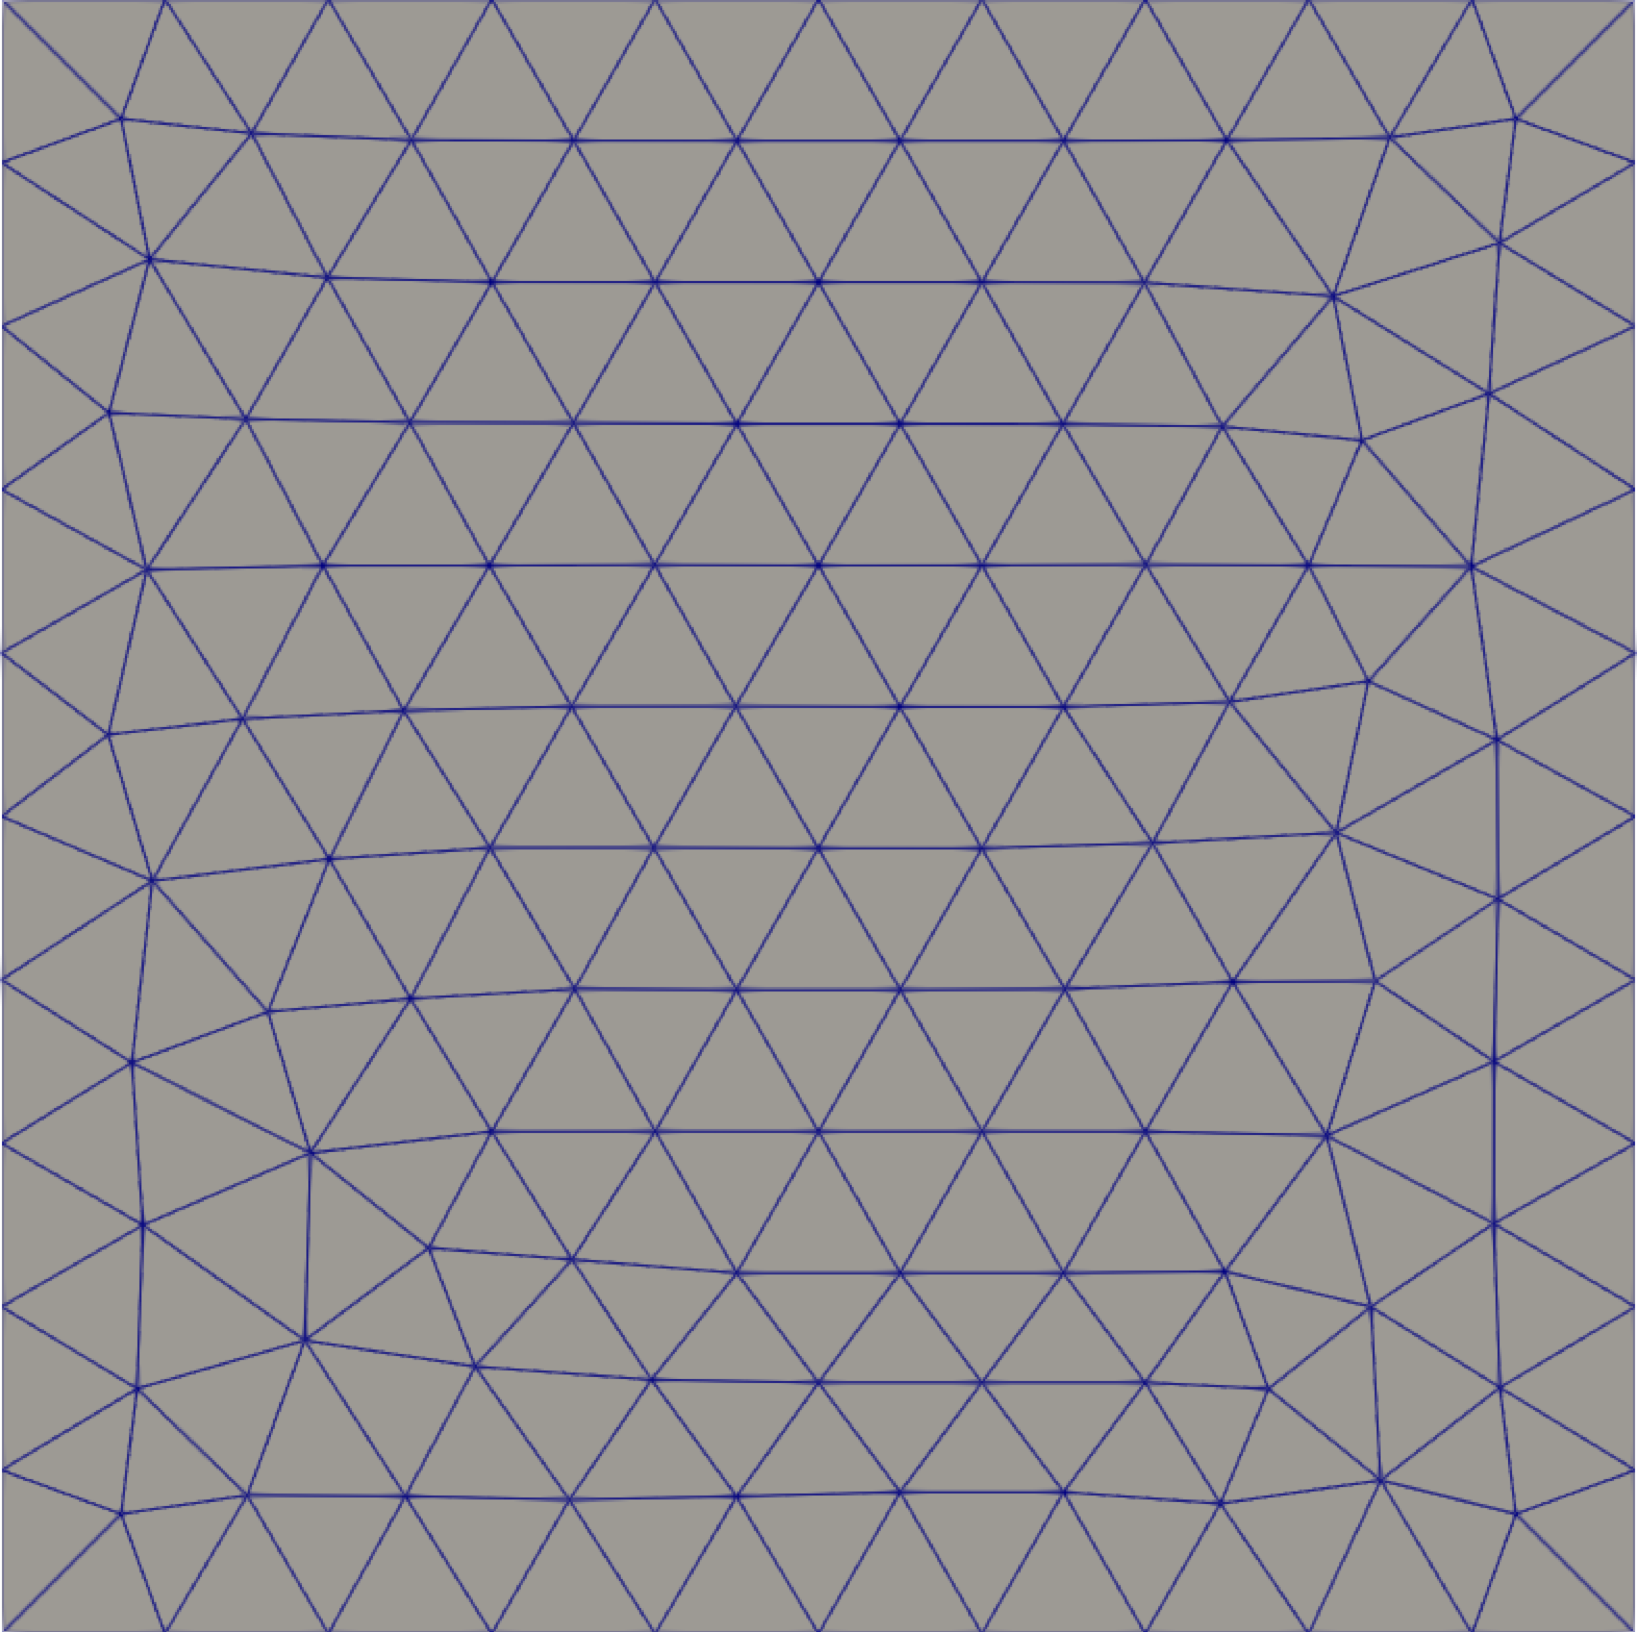
\includegraphics[width=\textwidth]{images/carre_euler_2.pdf}
    %\caption{Maillage quadrilatéral.}
    %\label{fig:mail_tri_vs_mail_quad_2}
\end{subfigure}
\caption{Illustration de l'invariance de la caractéristique d'Euler. A gauche on a une triangulation de 30 sommets, 71 arêtes et 42 triangles ($\chi(\Sigma)=1$) et à droite, on a une triangulation de 142 sommets, 383 arêtes et 242 triangles ($\chi(\Sigma)=1$).}
\label{fig:carre_euler}
\end{figure}
\begin{definition}[\cite{Henri_Paul_de_Saint_Gervais}]
Soit $\Sigma$ une surface compacte. Notons $S$, $A$ et $F$ le nombre de sommets, arêtes et faces d'une décomposition polyédrale de $\Sigma$. Alors le nombre
$$
S-A+F,
$$
est indépendant du choix de cette décomposition polyédrale. On l’appelle caractéristique d’Euler de $\Sigma$ et on la note $\chi(\Sigma)$.
\end{definition}

La caractéristique d'Euler d'une surface orientable $\Sigma$ peut être calculée à partir de son genre $g$ et du nombre $b$ de composante connexe de son bord \cite{vallet:tel-01748689}:
$$
\chi(\Sigma) = 2-2g-b.
$$
Pour les variétés riemanniennes, la caractéristique d'Euler peut également être trouvée en intégrant la courbure à partir du théorème de Gauss-Bonnet. Ainsi si $\Sigma$ est une variété Riemanienne compact alors on a \cite{lee2018introduction}:
$$
\displaystyle\int_\Sigma KdA+\int_{\partial\Sigma} k_{g}\,ds=2\pi \chi (\Sigma)
$$
Ici, $\partial\Sigma$ désigne le bord de $\Sigma$, $K$ la courbure gaussienne de $\Sigma$ et $k_g$ la courbure géodésique de $\partial\Sigma$. $dA$ est l'élément d'aire de la surface, et $ds$ est l'élément de ligne le long du bord de $\Sigma$.

Nous illustrons l'invariance de la caractéristique d'Euler sur la figure \ref{fig:carre_euler} avec deux triangulation différente d'un même domaine. Dans ce cas la caractéristique d'Euler vaut 1 avec $g=0$ et $b=1$.


\chapter{Opérateur Laplacien discret}
\label{Op_lap_discr}

L'opérateur Laplace-Beltrami $\Delta$ joue un rôle central dans les algorithmes géométriques appliqués aux domaines courbes. La formule des cotangentes, exposée dans \cite{operatorlecture, crane2019n}, offre une approche pratique pour approximer cet opérateur sur des surfaces triangulées bidimensionnelles. Considérons la résolution de l'équation de Poisson
\[ \Delta u = f, \]
sur une surface courbée $\Omega$. Ici, $f : \Omega \rightarrow \mathbb{R}$ représente une fonction source, $u : \Omega \rightarrow \mathbb{R}$ est une fonction inconnue, et $\Delta$ désigne l'opérateur Laplace-Beltrami associé à $\Omega$, également appelé le laplacien. Une approche courante pour approximer la solution fait appel au concept de solution faible. Les solutions faibles pour l'équation de Poisson sont des fonctions $\phi$ qui satisfont à l'ensemble d'équations suivant :
\[ \int_{\Omega} \phi \Delta u \,dA = \int_{\Omega} \phi f \,dA, \quad \forall \text{ fonctions tests } \phi .\]
Il est important de souligner que, selon la méthode de Galerkin, le choix des fonctions de base pour $u$, $f$, et la fonction test $\phi$ est essentiel. Ainsi, nous avons besoin d'un ensemble de fonctions de base sur $\Omega$. Pour une surface triangulée, les fonctions chapeau linéaires par morceaux $h_i$ se révèlent être le choix le plus naturel. Elles sont définies de manière à valoir un au sommet associé et zéro à tous les autres sommets. Par conséquent, si nous connaissons la valeur de $u(x)$ sur chaque sommet $v_i$, $u(v_i) = u_i$, nous pouvons l'approximer de la manière suivante :
\[ u(x) = \sum_{i} u_ih_i(x) .\]
De même, pour la fonction source $f$, nous avons :
\[ f(x) = \sum_{i} f_ih_i(x). \]
Avec la discrétisation de $u$ et $f$, en utilisant $h_i$ comme fonctions tests, nous pouvons maintenant exprimer le problème de Poisson d'origine comme un ensemble de $|V|$ équations :
\[ \int_{\Omega} h_i\Delta u \,dA = \int_{\Omega} h_if \,dA, \quad \forall i \in \{1, 2, . . . , |V|\},\]
où $|V|$ représente le nombre de sommets dans la triangulation.
 Ainsi on a:
\begin{equation}
\left\{
\begin{array}{l}
    \displaystyle\int_{\Omega} h_i\Delta u \,dA = - \int_{\Omega} \nabla h_i \cdot \nabla u \,dA = - \int_{\Omega} \nabla h_i \cdot \nabla \left(\sum_{j} u_j h_j\right) \,dA = - \sum_{j} u_j \int_{\Omega} \nabla h_i \cdot \nabla h_j \,dA,\\\\
    \displaystyle\int_{\Omega} h_if \,dA = \int_{\Omega} h_i \cdot \left(\sum_{j} b_j h_j\right) \,dA = \sum_{j} f_j \int_{\Omega} h_i \cdot h_j \,dA.
\end{array}
\right.
\end{equation}
Soit \(L\) la matrice \(L = \{L_{ij}\}^{|V|\times|V|}\), \(L_{ij} = \displaystyle\int_{\Omega} \nabla h_i \cdot \nabla h_j \,dA\) et \(M\) la matrice \(M = \{M_{ij}\}^{|V|\times|V|}\), \(M_{ij} = \displaystyle\int_{\Omega} h_i \cdot h_j \,dA\). On a alors le problème linéaire:
$$
L\mathbf{u}=M\mathbf{f},
$$
avec
\[
\mathbf{u}=\begin{bmatrix}
u_1\\
u_2\\
\vdots \\
u_{|V|}
\end{bmatrix}
\quad\quad\quad\mbox{ et }\quad\quad\quad
\mathbf{f}=
\begin{bmatrix}
f_1\\
f_2\\
\vdots \\
f_{|V|}
\end{bmatrix}.
\]
Pour calculer la matrice \(L\), nous examinons les éléments \(L_{ij} = \displaystyle\int_{\Omega} \nabla h_i \cdot \nabla h_j \,dA\), dont l'évaluation équivaut au calcul de l'intégrale sur chaque triangle, suivi de la sommation des résultats obtenus sur l'ensemble des triangles de \(\Omega\). Étant donné que \(h_i\) est une fonction linéaire par morceau sur chaque triangle, le calcul sur un triangle donné revient à multiplier le scalaire \(\nabla h_i \cdot \nabla h_j\) sur ce triangle par la surface du triangle. Nous allons maintenant examiner le gradient d'une fonction linéaire sur un triangle.

Soit \(g\) une fonction linéaire définie sur un triangle \(T\) de sommets \(v_1\), \(v_2\), \(v_3\) et d'aire \(A\) avec \(g(v_1) = 1\), \(g(v_2) = g(v_3) = 0\). \(g\) étant linéaire, on a \(g(x) = g(x_0) + \nabla g |_{x_0} \cdot (x - x_0)\) pour tout \(x\) appartenant au triangle.
Sachant que \(\nabla g \cdot (v_1 - v_3) = 1\) et \(\nabla g \cdot (v_2 - v_3) = 0\), il vient que \(\nabla g\) est perpendiculaire à l'arête \(v_2v_3\) et on a d'une part:
\[
||\nabla g|| \|\overrightarrow{v_1v_3}\| \cos\left(\displaystyle\frac{\pi}{2} - \theta\right) = ||\nabla g|| \|\overrightarrow{v_1v_3}\| \sin \theta=1,
\]
où $\theta$ désigne l'angle orienté entre les vecteurs $\overrightarrow{v_1v_3}$ et $\overrightarrow{v_2v_3}$. Autrement dit,
\begin{equation}
||\nabla g||=\frac{1}{h},
\label{eqn:ca_passe}
\end{equation}
et d'autre part:
\begin{equation}
\nabla g= \displaystyle\frac{\overrightarrow{v_2v_3}^\perp}{2\mathcal{A}},
\label{eqn:ca_casse}
\end{equation}
où $\mathcal{A}=\displaystyle\frac{1}{2} \|\overrightarrow{v_2v_3}\|h$ désigne l'aire du triangle et $h$ est la hauteur passant par $v_1$ et perpendiculaire au côté $v_2v_3$ avec \(\overrightarrow{v_2v_3}^\perp\) la rotation dans le sens anti-horaire de \(\overrightarrow{v_2v_3}\) d'angle \(\pi/4\).

On peut maintenant évaluer
$$\displaystyle\int_{T} \nabla h_i \cdot \nabla h_j dA,$$
où $T$ désigne un triangle du maillage.

Pour $i=j$, on a:
\[
\begin{array}{lcl}
\displaystyle\int_T \langle \nabla h_i, \nabla h_i \rangle dA &= &\mathcal{A}||\nabla h_i||^2
\end{array}
\]
En utilisant l'équation \ref{eqn:ca_passe}, on obtient:
\[
\displaystyle\int_T \langle \nabla h_i, \nabla h_i\rangle dA = \mathcal{A}\displaystyle\frac{1}{h^2}= \displaystyle\frac{b}{2h}
\]
où \(h\) désigne la hauteur passant par le sommet en question et \(b\) est la longueur du côté opposé à ce sommet (voir figure \ref{fig:laplace_cotan_1}). On se retrouve alors avec la formule :
\[
\begin{array}{lcl}
\displaystyle\int_T \langle \nabla h_i, \nabla h_i \rangle dA  &=& \displaystyle\frac{h \cot \theta_j^{ki} + h \cot \theta_k^{ij}}{2h}\\\\
\displaystyle\int_T \langle \nabla h_i, \nabla h_i\rangle dA&=& \displaystyle\frac{1}{2} (\cot \theta_j^{ki} + \cot \theta_k^{ij})
\end{array}
\]
En notant \(\alpha\) et \(\beta\) les angles intérieurs aux deux autres sommets du triangle (voir figure \ref{fig:laplace_cotan_1}).
\begin{figure}[!h]
\centering
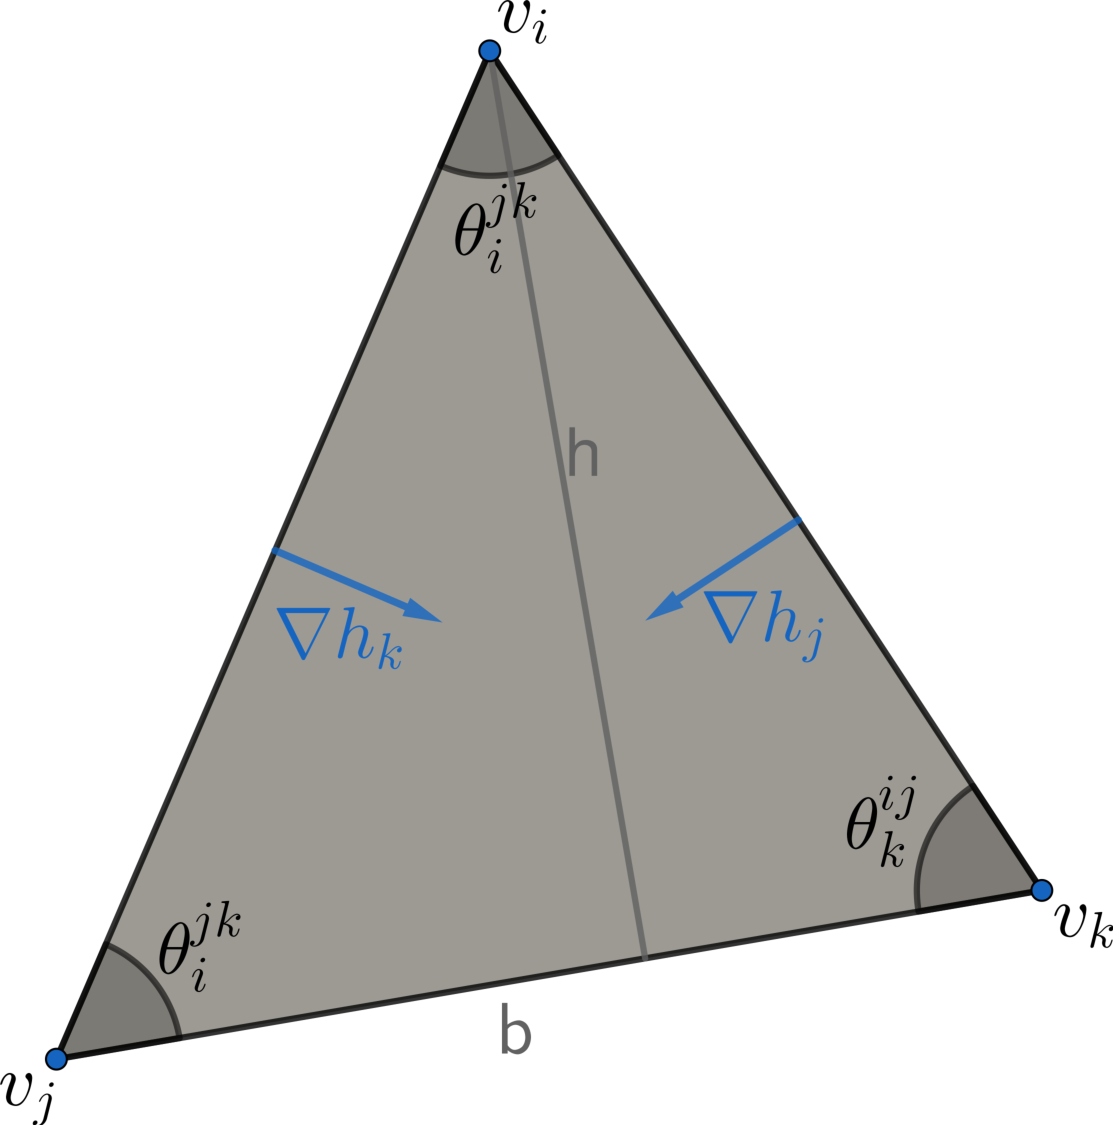
\includegraphics[scale=0.48]{images/laplace_cotan_1.pdf}
\caption{Cas où les sommets sont identiques.}
\label{fig:laplace_cotan_1}
\end{figure}

Regardons maintenant le cas où on a $i\neq j$ avec $v_i$ et $v_j$ appartenant à une même arête. On a:

\[
\begin{array}{lcl}
\displaystyle\int_T \langle \nabla h_i, \nabla h_j \rangle dA &= &\mathcal{A}\langle \nabla h_i, \nabla h_j \rangle
\end{array}
\]
En utilisant l'équation \ref{eqn:ca_casse}, on obtient:
\[
\begin{array}{lcl}
\displaystyle\int_T \langle \nabla h_i, \nabla h_j \rangle dA&=& \displaystyle\frac{1}{4\mathcal{A}} \langle \overrightarrow{v_kv_i}^\perp, \overrightarrow{v_iv_j}^\perp \rangle
\end{array}
\]
En adoptant les notations de la figure \ref{fig:laplace_cotan_1}, il vient:
\[
\begin{array}{lcl}
\displaystyle\int_T \langle \nabla h_i, \nabla h_j \rangle dA&=& -\displaystyle\frac{\|\overrightarrow{v_kv_i}\|\|\overrightarrow{v_iv_j}\| \cos \theta_i^{jk}}{4\mathcal{A}}\\\\
&=& -\displaystyle\frac{(h/\sin \theta_j^{ki})(h/\sin \theta_3^{12}) \cos \theta_i^{jk}}{2bh}\\\\
&=& -\displaystyle\frac{h \cos \theta_i^{jk}}{2(h \cot \theta_j^{ki} + h \cot \theta_k^{ij}) \sin \theta_j^{ki} \sin \theta_k^{ij}}\\\\
&=& -\displaystyle\frac{\cos \theta_i^{jk}}{2(\cos \theta_j^{ki} \sin \theta_k^{ij} + \cos \theta_k^{ij} \sin \theta_j^{ki})}\\\\
&=& -\displaystyle\frac{\cos \theta_i^{jk}}{2 \sin(\theta_j^{ki} + \theta_k^{ij})}\\\\
&=& -\displaystyle\frac{\cos \theta_i^{jk}}{2 \sin \theta_i^{jk}}\\\\
\displaystyle\int_T \langle \nabla h_i, \nabla h_j \rangle dA&=& -\displaystyle\frac{1}{2}\cot \theta_i^{jk}
\end{array}
\]
Enfin lorsque $i\neq j$ et que $v_i$ et $v_j$ n'appartiennent pas à une même arête, on a:
$$\displaystyle\int_T \langle \nabla h_i, \nabla h_j \rangle dA=0.$$

\begin{figure}[!h]
\begin{subfigure}{0.46\textwidth}
    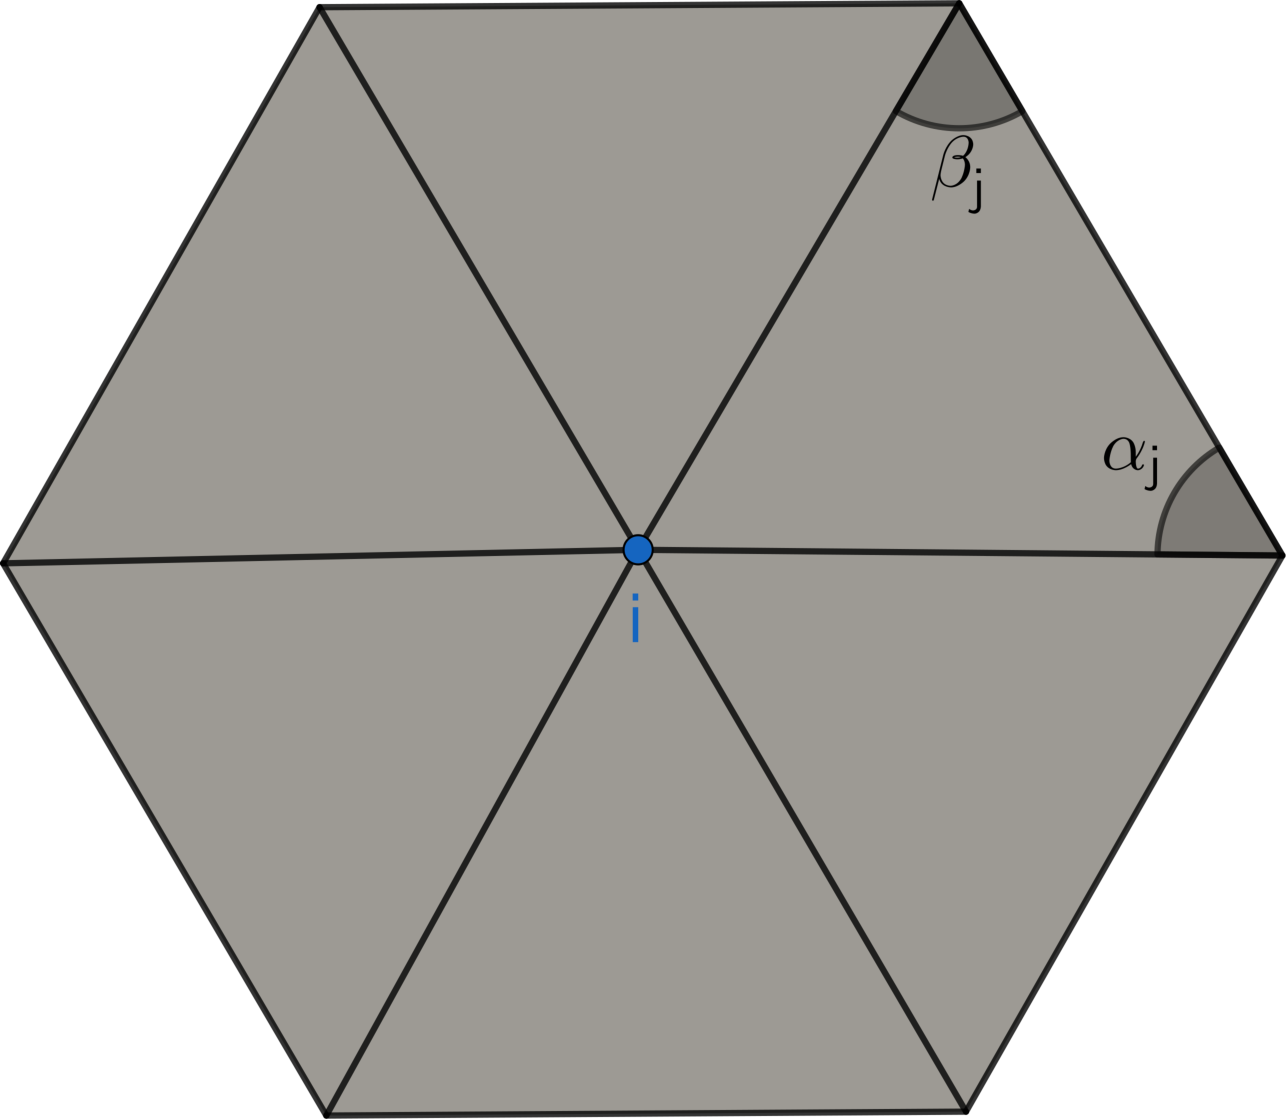
\includegraphics[width=\textwidth]{images/laplace_cotan_3.pdf}
    %\caption{Maillage triangulaire.}
    %\label{fig:mail_tri_vs_mail_quad_1}
\end{subfigure}
\hfill
\begin{subfigure}{0.46\textwidth}
    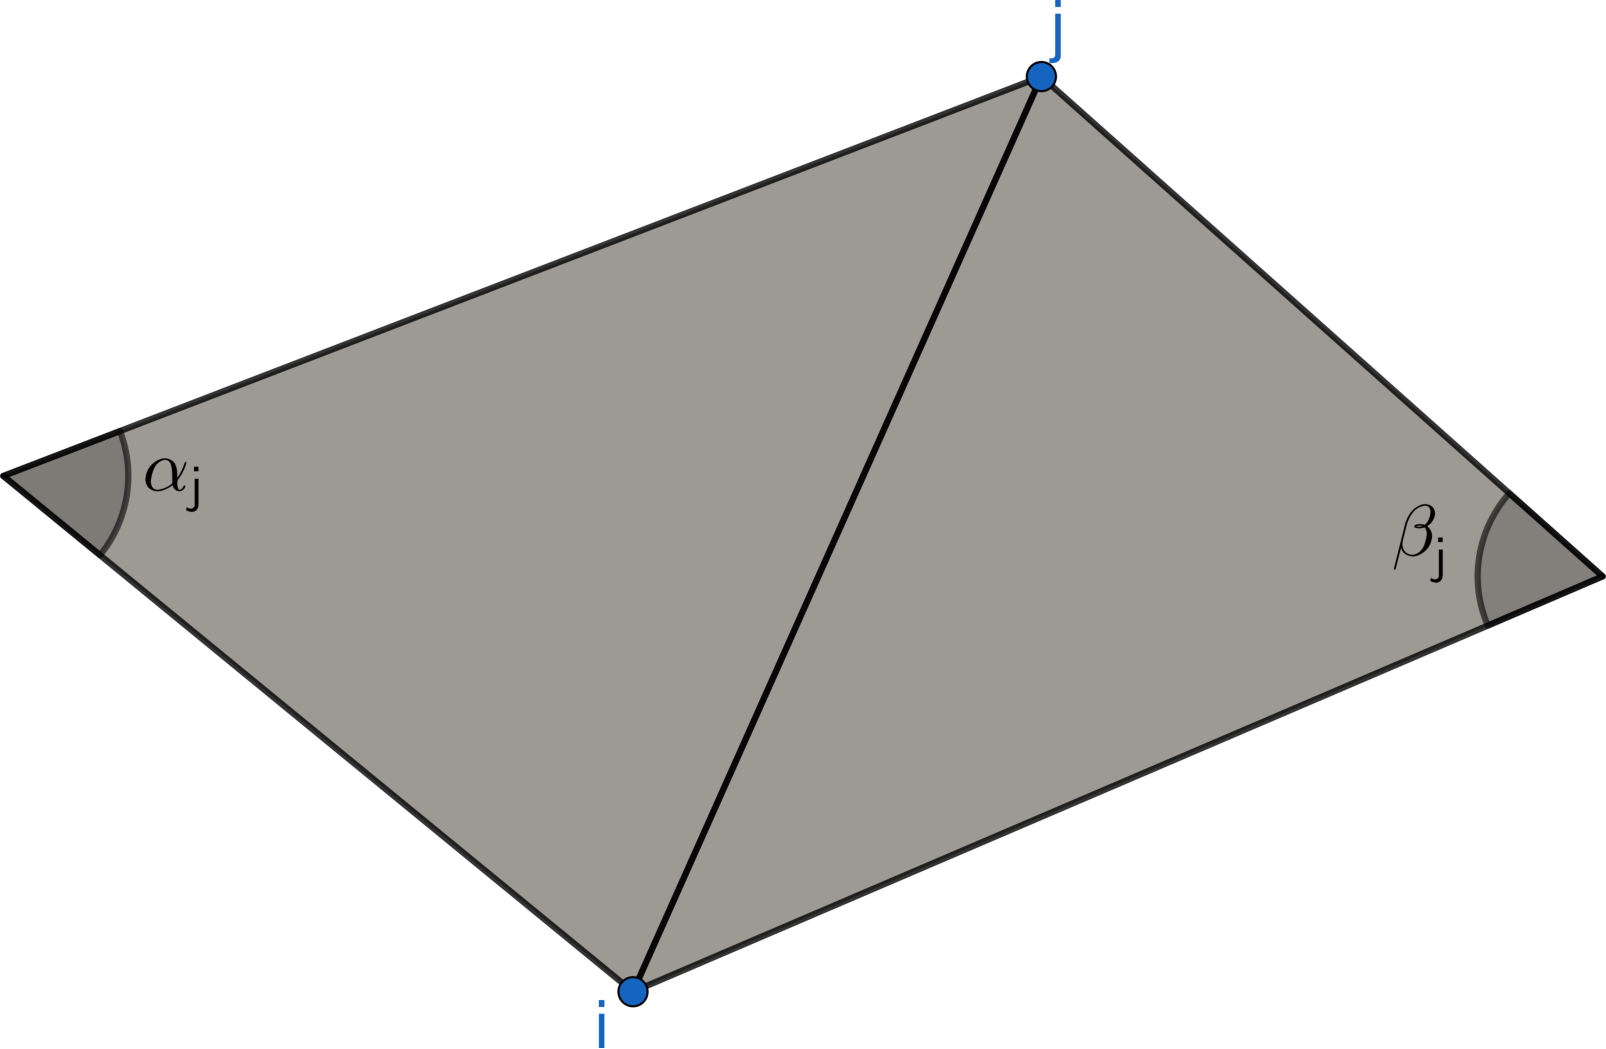
\includegraphics[width=\textwidth]{images/laplace_cotan_2.pdf}
    %\caption{Maillage quadrilatéral.}
    %\label{fig:mail_tri_vs_mail_quad_2}
\end{subfigure}
\caption{Somme autour des sommets.}
\label{fig:laplace_cotan_cotan}
\end{figure}

En sommant ces résultat sur tous les triangles et en adoptant les notations de la figure \ref{fig:laplace_cotan_cotan}, on obtient:
\[
L_{ij} =\displaystyle\int_\Omega \langle \nabla h_i, \nabla h_j \rangle dA=
\begin{cases}
\displaystyle\frac{1}{2} \sum_{k\sim i} (\cot \alpha_j + \cot \beta_j), & \text{si } i = j, \\\\
-\displaystyle\frac{1}{2} (\cot \alpha_j + \cot \beta_j), & \text{si } j \sim i, \\\\
0, & \text{sinon}.
\end{cases}
\]
où $i \sim j$ signifie que les sommets $v_i$ et $v_j$ sont adjencents. On se ramène ainsi à une construction simple basée juste sur les informations géométriques (les angles) du maillage.


\chapter{Une approche pour la discrétisation du problème d'adaptation}
\label{discr_adapt}
Pour une question d’efficacité nous allons remplacer la résolution du problème d’optimisation globale \eqref{eqn:adapt_eqn_1} en une série d’optimisations locales. L’idée est de procéder triangle par triangle en notant que la contrainte de bord permet de définir explicitement la valeur de $\alpha$. La formulation éléments finis de \eqref{eqn:adapt_eqn_1} avec cette contrainte revient à trouver $\alpha_h\in\mathbb{P}_1(\Omega)$ tel que:
\begin{equation}
\begin{cases}
\tilde{\theta}_h := \theta_h + \alpha_h \in P^1(\Omega), \\\\
\min \left|\theta_h - \tilde{\theta}_h\right|, \\\\
\alpha_h = \phi_h - \theta_h, \ \partial\Omega, \\\\
\text{Supp}\,\alpha_h \subset V, \\\\
\|\nabla\alpha_h\| \leq \nu.
\end{cases}
\label{eqn:adapt_eqn_2}
\end{equation}
En pratique, la résolution de \eqref{eqn:adapt_eqn_2} peut être effectuée via la construction locale de $\tilde{\theta}_h$ sur chaque triangle $T\in\mathcal{T}_h$ suivante:\\
\begin{enumerate}
    \item Affectation des valeurs $\tilde{\theta}_h(S) = \phi_h(S)$ pour tous les nœuds $S \in \partial\Omega$,\\
    \item Tant qu'il reste des triangles à traiter :\\
    \begin{enumerate}
        \item Suppression des triangles ayant déjà $\tilde{\theta}_h$ calculé sur les 3 nœuds de la liste des triangles à traiter,\\
        \item Recherche des triangles $T$ pour lesquels $\tilde{\theta}_h$ est définie pour 2 nœuds sur 3,\\
        \item Si les valeurs de $\tilde{\theta}_h$ pour 2 nœuds sur 3 de $T$ sont nulles alors $T$ est retiré de la liste à évaluer,\\
        \item Sur $T_h$ on note $S_1$ et $S_2$ les nœuds pour lesquels $\tilde{\theta}_h$ a été évaluée, $S_3$ le troisième sommet, $\overrightarrow{h_3}$ la hauteur normalisée issue de $S_3$, $X_h = x_hS_2 +(1-x_h)S_1$ le pied de la hauteur et $h_3 = |X_h - S_3|$,\\
        \item À partir d'une valeur $\tilde{\theta}_h(S_1) \left[ \frac{\pi}{2} \right]$, on calcule
        \[
        \tilde{\theta}_h(S_2, S_1) := \arg\min_{y\in{\tilde{\theta}_h(S_2)+k\pi/2, k\in\mathbb{Z}}}
        \left|y - \tilde{\theta}_h(S_1)\right|,
        \]
        et on note $\beta = x_h \tilde{\theta}(S_2, S_1) + (1 - x_h)\tilde{\theta}(S_1)$,\\
        \item Calcul des variations maximales possibles pour $\theta \in [\theta^-, \theta^+]$ :
        \[
        \theta^\pm = \beta \pm |h_3|\nu\overrightarrow{h_3}.
        \]
        \item La solution est alors simplement obtenue par
    \[
    \tilde{\theta}_h(S_3) = \min(\theta^+, \max(\theta^-, \theta_h(S_3))),
    \]
    et le triangle est marqué comme traité.
    \end{enumerate}
\end{enumerate}
La fonction $\alpha_h = \tilde{\theta}_h - \theta_h$ vérifie alors les propriétés attendues dans \eqref{eqn:adapt_eqn_2}. Concernant le choix de $\nu$, on prend typiquement
\[
\nu = \frac{\pi}{4d} \mbox{ avec } d = nh,
\]
où $h$ est une grandeur caractéristique du maillage (typiquement la hauteur minimale) et $n > 0$. Cela porte le support de $\alpha_h$ typiquement à $d$ de $\partial\Omega$. Le $\pi/4$ représente la valeur maximale de variation attendue sur les angles, vu qu’ils sont définis par modulo $\pi/2$.


\chapter{Algorithme de coloriage}
\label{algo_glouton}


Nous exposons ici un algorithme qui permet l'identification des parties connexes d'un maillage en attribuant une marque (couleur) aux triangles appartenant à une même partie connexe.


\RestyleAlgo{ruled}
\begin{algorithm}[h!]
\renewcommand{\algorithmcfname}{Algorithme}%
\SetAlgoLined
\Entree{Maillage}
\Sortie{Marquage des triangle par composante connexe}
\vspace{0.15cm}
1.\quad Marquer tous les triangle à 0\\[0.15cm]
2.\quad Soit M=1\\[0.15cm]
\Tq{tous les triangles ne sont pas marqués}{
\vspace{0.15cm}
3.\quad Soit $V$ une liste vide\\[0.15cm]
4.\quad Stocker dans $V$ un triangle non marqué\\[0.15cm]
5.\quad Marqué le triangle Stocké avec M\\[0.15cm]
\Tq{$V$ n'est pas vide}{
\vspace{0.15cm}
6.\quad Soit $C=V$\\[0.15cm]
7.\quad Vider $V$\\[0.15cm]
\SetKwFor{PourCh}{pour chaque}{faire}{fin pour chaque}%
\PourCh{triangle $T$ dans $C$}{
\vspace{0.15cm}
\PourCh{arête $a$ de $T$}{
\vspace{0.15cm}
\Si{$a$ n'est pas une arête de bord et que le triangle voisin à $T$ par rapport à $a$ n'est pas marqué}{
\vspace{0.15cm}
8.\quad Stocker dans $V$ un triangle voisin\\[0.15cm]
9.\quad Marqué le triangle Stocké avec M\\[0.15cm]
}
\vspace{0.15cm}
}
\vspace{0.15cm}
}
\vspace{0.15cm}
}
\vspace{0.15cm}
10.\quad M=M+1\\[0.15cm]
}
\caption{Algorithme de coloriage}
\label{alg:coloriage}
\end{algorithm}




%theoreme des tangentes tournantes
%Algorithme glouton pour le partitionnement en sous maillage
